\documentclass[manuscript,screen,review]{acmart}
\usepackage{booktabs}
\usepackage{tabularx}
\usepackage{array}
\usepackage{ragged2e}
\usepackage{float}

% Custom column types
\newcolumntype{L}{>{\RaggedRight\arraybackslash}X}
\newcolumntype{C}{>{\Centering\arraybackslash}X}

\AtBeginDocument{%
  \providecommand\BibTeX{{Bib\TeX}}}

\begin{document}

%% =================== TITLE & AUTHOR BLOCK =========================
\title{FairLab: A Fairness-Aware Workstation Booking, Allocation, and Access-Control System}
\subtitle{Computer Systems Design Project Report --- Group 10 (IIT Bhilai Lab L-106)}

\author{Ganesh}
\affiliation{%
  \institution{Department of Computer Science and Engineering, IIT Bhilai}
  \city{Bhilai}
  \country{India}}
\email{ganesh.k@iitbhilai.ac.in}

\author{V Karthik}
\affiliation{%
  \institution{Department of Computer Science and Engineering, IIT Bhilai}
  \city{Bhilai}
  \country{India}}
\email{vkarthik@iitbhilai.ac.in}

\author{Charith Reddy}
\affiliation{%
  \institution{Department of Computer Science and Engineering, IIT Bhilai}
  \city{Bhilai}
  \country{India}}
\email{charithr@iitbhilai.ac.in}

\renewcommand{\shortauthors}{Ganesh, V Karthik, and Charith Reddy}

%% =================== ABSTRACT ======================================
\begin{abstract}
Shared academic computer laboratories suffer from severe allocation skew during project deadlines and examination periods when governed by First-In-First-Out (FIFO) booking queues. Fast-clicking users and automated scripts monopolize workstations, starving regular students while existing tools lack physical gate verification and academic timetable integration. We design, implement, and deploy \textbf{FairLab}, a fairness-aware workstation booking, allocation, and physical access-control platform tailored to IIT Bhilai Computer Lab L-106 (84 workstations across Block~A $6\times 10$ and Block~B $4\times 6$). FairLab combines half-open time intervals $[start, end)$ enforced by database-level non-overlap constraints, a hybrid immediate-versus-fairness allocation engine with atomic contention detection, configurable institutional scheduling policies (2-hour limit, Monday--Friday class timetables, holiday overrides, and ticket releases), zero-trust HS256 JWT authentication with scoped \texttt{ACCESS\_OPERATOR} gate permissions, zero-PII HMAC-SHA256 QR passes, and a Transactional Outbox with cross-replica WebSocket fan-out. Deployed on Group~10's campus VM behind an Nginx load balancer routing across two PM2 Node.js replicas, FairLab passes 14/14 automated test suites (including 76 acceptance assertions and live PostgreSQL~16 checks). In a 50-seed deterministic benchmark under bot-latency skew, FairLab reduces allocation Gini inequality from $0.657$ (FIFO) to $0.022$ and raises Jain's Fairness Index from $0.252$ to $0.998$.
\end{abstract}

\keywords{Fair Scheduling, Resource Allocation, Concurrency Control, Transactional Outbox, Role-Based Access Control}

\maketitle

%% =====================================================================
\section{Introduction}
\label{sec:intro}
Shared departmental computing laboratories such as IIT Bhilai's Computer Lab L-106 provide 84 high-utility workstations serving hundreds of undergraduate, M.Tech., and Ph.D.\ students across coursework, assignments, and research. Under conventional First-In-First-Out (FIFO) reservation portals or manual spreadsheets, seat allocation correlates with submission speed rather than equitable access. During peak academic weeks, repeated heavy users or scripted polling bots capture scarce slots within milliseconds, causing long wait times and frustration among regular students. Simultaneously, labs require operational enforcement of recurring weekday class timetables, ad-hoc holidays, physical gate verification to deter proxy attendance and no-shows, and resilient handling of workstation maintenance.

This report presents \textbf{FairLab}, an end-to-end full-stack system engineered specifically for Lab L-106. FairLab replaces FIFO contention with a transparent, history-aware fairness scoring model, enforces non-overlapping reservations directly inside the database layer, separates administrative policy configuration from physical gate verification through scoped permissions, and runs live on our assigned campus VM with load-balanced backend replicas.

The remainder of this report is organized as follows: Section~\ref{sec:requirements} defines functional and non-functional requirements; Section~\ref{sec:architecture} presents the system architecture and technology stack; Section~\ref{sec:methodology} details the fairness algorithm, hybrid allocation protocol, and validation methodology; Section~\ref{sec:implementation} describes backend APIs, frontend views, and storage; Section~\ref{sec:csd-themes} maps core Computer Systems Design (CSD) themes to concrete modules; Section~\ref{sec:results} reports test and benchmark results; Section~\ref{sec:discussion} reflects on limitations and future work; and Section~\ref{sec:ai-usage} provides our AI tool usage declaration.

\subsection{Motivation}
Existing reservation tools exhibit four structural gaps in an academic lab setting: (1)~FIFO allocation permits bot-driven hoarding and offers no penalty for repeated no-shows or credit for prior waiting; (2)~application-only availability checks are vulnerable to double-booking race conditions under simultaneous clicks; (3)~flat admin roles either expose sensitive gate check-in actions to all faculty or introduce unnecessary role proliferation; and (4)~most booking prototypes ignore recurring Mon--Fri academic lab schedules and holiday overrides. FairLab addresses all four gaps using principled systems-engineering mechanisms while keeping the user experience immediate whenever a time window is uncontested.

\subsection{Scope of the Project}
\textbf{Included in FairLab v1.0.0:} Complete 84-workstation inventory (Block~A $6\times 10$ + Block~B $4\times 6$); custom half-open interval booking $[start, end)$ ($30\text{ min}$--$2\text{ h}$) with 1--3 ranked workstation preferences; hybrid immediate/fairness allocation with atomic anti-bypass checks; configurable Mon--Fri academic timetable blocks, holiday/extra-day overrides, and ticket release caps; zero-trust HS256 JWT + \texttt{HttpOnly} cookie authentication (\texttt{@iitbhilai.ac.in}); strictly two roles (\texttt{student}, \texttt{admin}) with scoped \texttt{ACCESS\_OPERATOR} gate permission; zero-PII HMAC-SHA256 QR verification with anti-replay check-in/out; automatic reallocation on workstation maintenance; Transactional Outbox with 1-second cross-replica WebSocket fan-out; 15-screen React SPA; 14 automated test suites; and live deployment on Group~10's campus VM.

\textbf{Explicitly Excluded (Planned Future Work):} Cryptographic mailbox ownership via IIT Bhilai Google Workspace OAuth/LDAP SSO (demo login currently validates domain suffix and registered accounts); physical L-106 turnstile door relays; live NVIDIA-SMI workstation GPU telemetry agents (UI honestly renders ``---'' with no synthetic readings); HTTPS TLS certificate provisioning on the private campus VM; and formal k6 load testing against PostgreSQL~16.

%% =====================================================================
\section{Problem Statement and Requirements}
\label{sec:requirements}
\textbf{Problem Statement:} Given a shared laboratory of $N=84$ workstations, $M$ competing student users, configurable institutional schedule restrictions, and concurrent HTTP requests, design a fault-tolerant reservation and gate-access system that prevents overlapping bookings at the database layer, allocates contested intervals fairly without permitting FIFO bypass, enforces least-privilege security, and maintains real-time consistency across load-balanced replicas. Table~\ref{tab:requirements} maps each functional requirement to its concrete implementation.

\begin{table}[htbp]
  \caption{Functional requirements and their implementation in FairLab}
  \label{tab:requirements}
  \small
  \begin{tabularx}{\columnwidth}{@{}p{0.38\columnwidth}L@{}}
    \toprule
    \textbf{Functional Requirement} & \textbf{Implementation / Evidence} \\
    \midrule
    FR1: 84-Seat Map \& Custom Interval Booking & \texttt{availabilityService.js} + \texttt{WorkstationMapView.jsx}; Block~A ($6\times 10$) \& Block~B ($4\times 6$), half-open $[start, end)$ ($30\text{m}$--$2\text{h}$), 1--3 ranked preferences. \\
    FR2: Hybrid Immediate vs.\ Fairness Allocation & \texttt{bookingService.js} (\texttt{immediateTx}) + \texttt{fairnessEngine.js}; atomic contention check prevents \texttt{AUTO} bypass; 4-tier fairness ranking on contested windows. \\
    FR3: Institutional Timetable, Holidays \& Tickets & \texttt{scheduleService.js} + \texttt{AdminScheduleView.jsx}; Mon--Fri class blocks, holiday/extra-day overrides, max 2h duration/daily quota, admin ticket release caps. \\
    FR4: Institute Auth \& Scoped Gate RBAC & \texttt{middleware/auth.js} + \texttt{routes/auth.js} + \texttt{routes/access.js}; \texttt{@iitbhilai.ac.in} HS256 JWT + cookie; 2 roles (\texttt{student}, \texttt{admin}) + \texttt{ACCESS\_OPERATOR} permission. \\
    FR5: Cryptographic QR Pass \& Gate Lifecycle & \texttt{passService.js} + \texttt{verificationService.js}; zero-PII \texttt{FAIRPASS:<id>:<hmac16>}, single-use \texttt{VALID} $\rightarrow$ \texttt{CHECKED\_IN} $\rightarrow$ \texttt{USED}, replay denial, check-out score deduction. \\
    FR6: Maintenance Reallocation \& Semester Reset & \texttt{gpuResourceService.js} (auto-moves active bookings off offline PCs) + \texttt{fairnessEngine.js} (archives term history, resets next-term scores to 100). \\
    \bottomrule
  \end{tabularx}
\end{table}

\subsection{Non-Functional Requirements}
\begin{itemize}
  \item \textbf{Consistency \& Zero Double-Booking:} Hard non-overlap invariants enforced inside SQLite triggers and PostgreSQL~16 \texttt{EXCLUDE USING gist} (\texttt{SQLSTATE 23P01}); idempotent retries via \texttt{Idempotency-Key}.
  \item \textbf{Security:} Constant-time HS256 JWT verification (\texttt{crypto.timingSafeEqual}); strict rejection of client-supplied \texttt{x-user-id} (\texttt{401}) and demo switches (\texttt{403}) in \texttt{NODE\_ENV=production}; Zod~v4 schema validation; 64\,KB payload cap; per-user sliding-window rate limiting (\texttt{429}); zero hardcoded secrets.
  \item \textbf{Performance \& Footprint:} Single-request API latency $<50\text{ ms}$ on campus VM; 100 concurrent submissions handled in $<250\text{ ms}$; cross-replica WebSocket event propagation $<1\text{ s}$ (measured $431\text{ ms}$); idle Node RSS $\approx 78$--$86\text{ MB}$ per replica, comfortably fitting a 10\,vCPU / 10\,GB RAM VM.
  \item \textbf{Reliability \& Recovery:} Transactional Outbox with startup + 5\,s crash recovery surviving hard \texttt{SIGKILL}; PM2 automatic worker restart; online SQLite hot backups and PostgreSQL \texttt{pg\_dump}.
\end{itemize}

%% =====================================================================
\section{System Architecture and High-Level Design}
\label{sec:architecture}
FairLab adopts a \textbf{layered modular monolith} deployed in a \textbf{two-replica load-balanced topology} on Group~10's Ubuntu~24.04 campus VM (\texttt{stu130\_sys1}, \texttt{10.1.75.40}, 10\,vCPU / 10\,GB RAM). Figure~\ref{fig:architecture} illustrates all layers and port mappings:

\begin{enumerate}
  \item \textbf{Client Layer (15-Screen React SPA):} Five student views (Dashboard, 84-Seat Map, My Bookings \& QR Pass, Fairness Ledger, Notifications), nine admin views (Overview, Allocation Round, Schedule \& Tickets, Workstations, Students, Analytics, Access Control, Settings, Audit Log), and Login.
  \item \textbf{Edge / Load Balancer Layer (Nginx 1.24):} Listens on container port \texttt{3000} (host \texttt{3500}) to serve the gzipped React bundle directly, proxy REST API traffic across two backend replicas using \texttt{least\_conn} with health failover (\texttt{max\_fails=3}), and terminate WebSocket upgrades on \texttt{/ws}. Port \texttt{4000} (host \texttt{4500}) exposes live Nginx \texttt{stub\_status} metrics.
  \item \textbf{Application Layer (Two PM2 Node.js Replicas):} \texttt{fairlab-api-1} (port \texttt{5000}$\rightarrow$\texttt{5500}) and \texttt{fairlab-api-2} (port \texttt{6000}$\rightarrow$\texttt{6500}) load identical runtime secrets (\texttt{JWT\_SECRET}, \texttt{HMAC\_SECRET}) from a \texttt{chmod 600} \texttt{.env} file so sessions and QR signatures validate seamlessly across replicas. Each replica houses modular domain services (Booking/Allocation, Fairness, Schedule/Timetable, QR Pass/Verification, Maintenance, Analytics) plus an atomic outbox publisher and a 1-second cross-replica outbox tailer.
  \item \textbf{Persistence \& Ops Monitoring Layer:} Both live API replicas share an ACID \textbf{SQLite WAL} database (\texttt{fairlab.db}, \texttt{busy\_timeout=5000\,ms}) with overlap triggers and transactional outbox rows. Alongside it, a live \textbf{PostgreSQL 16.15} cluster (\texttt{fairlab\_db}, 18 tables, \texttt{btree\_gist}) runs on port \texttt{5432} and is verified by live integration suites, ready for full async \texttt{pg}-pool runtime cutover. A dedicated PM2 operations dashboard (\texttt{7000}$\rightarrow$\texttt{7500}) continuously probes Nginx, both replicas, SQLite WAL, and PostgreSQL~16.
\end{enumerate}

\begin{figure}[H]
  \centering
  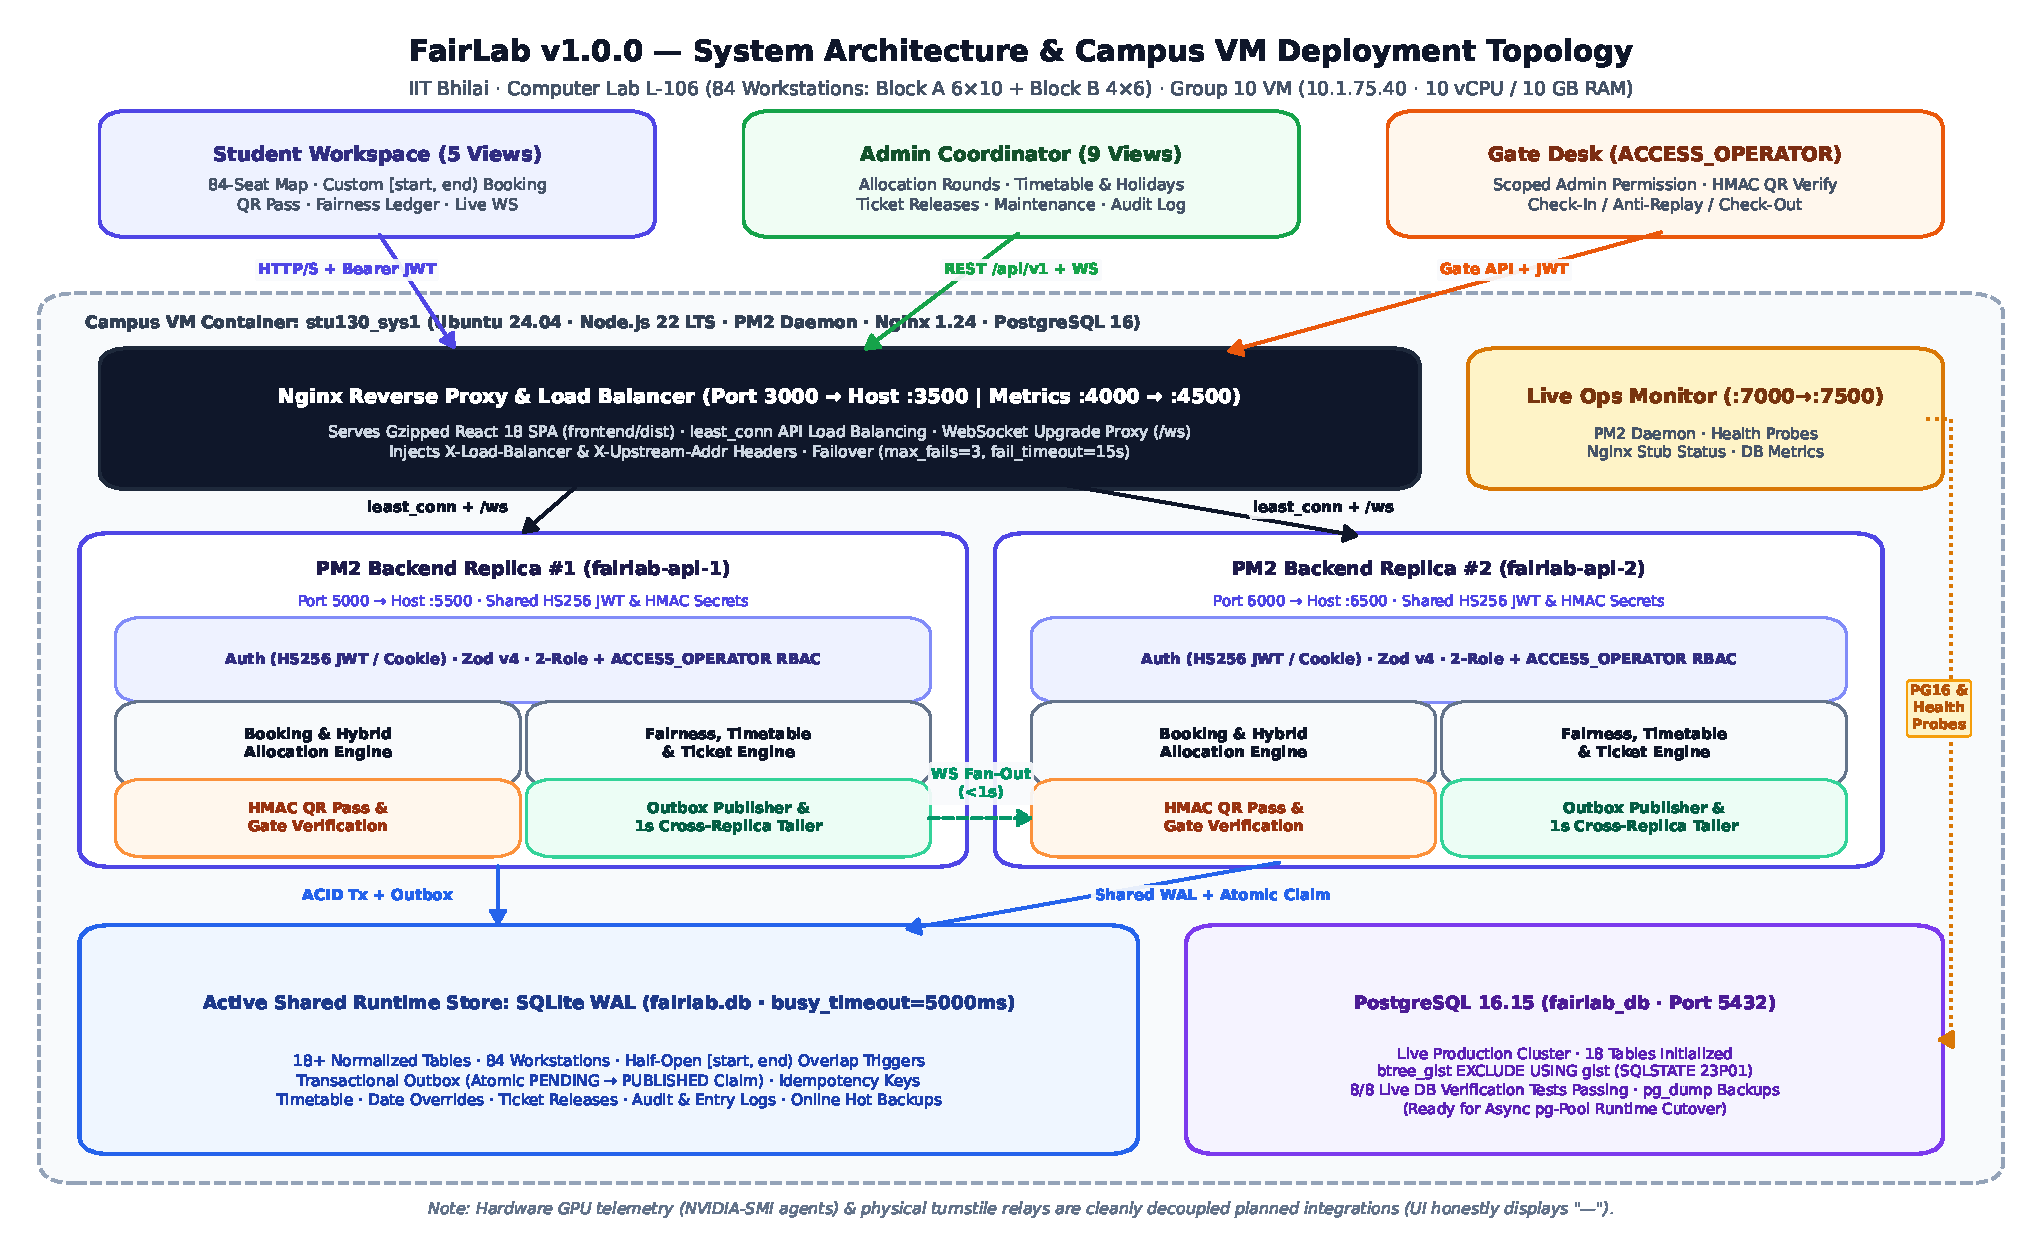
\includegraphics[width=0.96\linewidth]{fairlab_architecture.pdf}
  \caption{FairLab v1.0.0 system architecture and deployed two-replica campus VM topology (\texttt{10.1.75.40}).}
  \label{fig:architecture}
  \Description{Layered diagram showing Student, Admin, and Gate Desk clients connecting through an Nginx load balancer on port 3000/3500 to two PM2 Node.js backend replicas on ports 5000/5500 and 6000/6500 with cross-replica WebSocket fan-out, backed by a shared SQLite WAL runtime store, a verified PostgreSQL 16.15 cluster, and a live operations monitor on port 7000/7500.}
\end{figure}

\subsection{Technology Stack}
\textbf{Frontend:} React~18, Vite~6, Tailwind CSS, native browser WebSocket API (chosen for fast static builds --- 308\,KB gzipped to 80\,KB --- and zero runtime proxy overhead behind Nginx).
\textbf{Backend:} Node.js~22 LTS, Express, Zod~v4 (strict runtime request validation), \texttt{ws} (WebSockets), \texttt{qrcode} (QR rendering), Node built-in \texttt{crypto} (zero-dependency HS256 JWT and HMAC-SHA256 signing).
\textbf{Storage \& Deployment:} \texttt{better-sqlite3} (WAL mode, synchronous ACID transactions, zero serialization bugs under single-node contention), PostgreSQL~16.15 + \texttt{pg} driver + \texttt{btree\_gist} (verified production schema), Nginx~1.24 (reverse proxy \& load balancer), PM2~7 (process supervision and automatic crash restart), Docker/Compose templates for portable reproduction. We intentionally rejected a multi-service microservices split because Lab L-106 serves 84 seats and $\sim$500--2,000 campus users, where ACID database transactions in a modular monolith provide stronger consistency with far lower operational complexity.

%% =====================================================================
\section{Methodology}
\label{sec:methodology}
FairLab's core methodology couples strict database invariants with a closed-loop fairness allocation workflow, summarized in Figure~\ref{fig:methodology}. Every booking request traverses identity verification, configurable institutional policy validation, half-open overlap enforcement, an atomic contention check, deterministic fairness ranking (when contested), transactional outbox publishing, and cryptographic physical gate verification.

\begin{figure}[H]
  \centering
  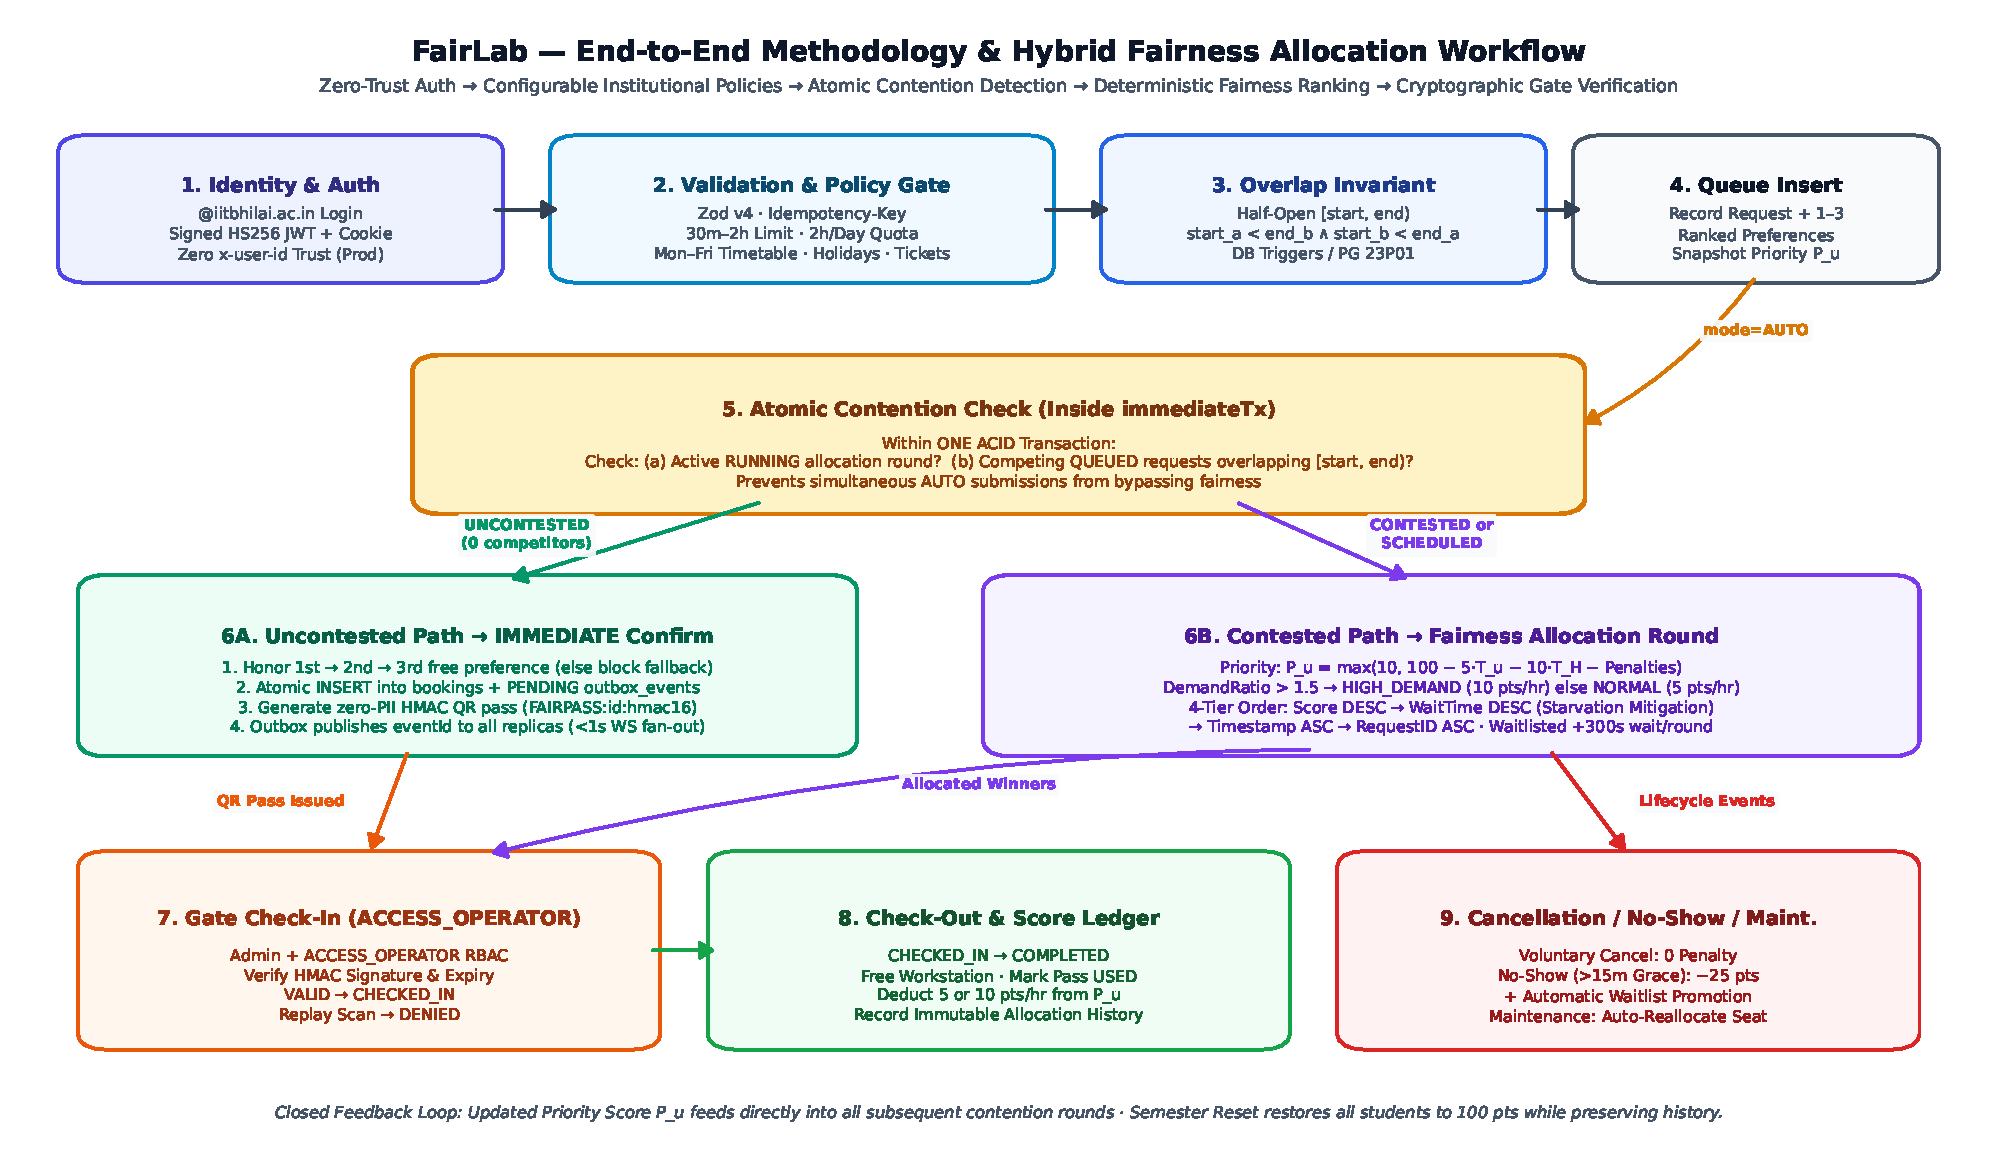
\includegraphics[width=0.96\linewidth]{fairlab_methodology.pdf}
  \caption{End-to-end FairLab methodology and hybrid immediate-versus-fairness allocation workflow.}
  \label{fig:methodology}
  \Description{Flowchart illustrating the 9-step lifecycle from IIT Bhilai HS256 JWT login, Zod and schedule/timetable validation, half-open interval overlap check, atomic contention decision inside immediateTx, uncontested immediate confirmation vs contested 4-tier fairness ranking, HMAC QR gate check-in, check-out score deduction, and cancellation/no-show/maintenance recovery.}
\end{figure}

\subsection{Data Collection and Preparation}
Lab L-106 physical layout data (84 workstations partitioned into Block~A rows 1--6 $\times$ 10 seats and Block~B rows 1--4 $\times$ 6 seats), recurring Monday--Friday academic lab course blocks (e.g., CS305, DS204), hourly default slots (09:00--18:00), ticket release templates, and representative IIT Bhilai personas (students, faculty coordinator, ordinary admin, and gate desk operator) are deterministically seeded by \texttt{backend/db/seed.js}. All calendar dates are validated against strict \texttt{YYYY-MM-DD} calendar existence (blocking invalid dates such as Feb~30 and past dates), and timestamps are normalized to canonical \texttt{HH:MM} half-open windows $[start, end)$.

\subsection{Analysis / Processing Method}
\textbf{Half-Open Interval Overlap Invariant:} Two reservations $[s_1, e_1)$ and $[s_2, e_2)$ on the same workstation and date conflict if and only if $s_1 < e_2 \land s_2 < e_1$. This allows seamless back-to-back sessions (e.g., 10:00--11:00 followed by 11:00--12:00) while mathematically prohibiting partial or total overlaps.

\textbf{Fairness Priority Scoring:} For each student $u$ in the active semester, FairLab maintains total completed hours $T_u$, high-demand completed hours $T_H$ (sessions allocated when $\text{DemandRatio} = \text{EligibleRequests} / \text{AvailableCapacity} > 1.5$), and accumulated no-show penalty points $\text{Penalties}_u$:
\begin{equation}
  P_u = \max\bigl(P_{\min},\; B - r_{\text{norm}}\cdot T_u - r_{\text{peak}}\cdot T_H - \text{Penalties}_u\bigr)
  \label{eq:fairness}
\end{equation}
Under default configurable policy ($B=100$, $P_{\min}=10$, $r_{\text{norm}}=5\text{ pts/hr}$, $r_{\text{peak}}=10\text{ pts/hr}$, no-show $=25\text{ pts}$, voluntary cancel $=0\text{ pts}$), heavy peak-hour users decline in priority faster than off-peak users, while voluntary early cancellation carries zero penalty to encourage releasing unused seats.

\textbf{Deterministic 4-Tier Contention Ordering:} Contested requests are sorted in $O(R\log R)$ time by: (1)~$P_u$ descending; (2)~cumulative eligible waiting time $W_u$ descending; (3)~submission timestamp ascending; and (4)~request ID ascending. Each unallocated waitlisted candidate accrues $+300\text{ s}$ of waiting time per round. \textit{Qualified Starvation-Mitigation Property:} Eligible waiting-time accumulation provides a starvation-mitigation mechanism among users with equal priority scores (including users at the floor $P_{\min}=10$); under sustained contention and defined eligibility assumptions, it progressively promotes users who have waited longer.

\textbf{Atomic Hybrid Contention Decision:} When a student submits an \texttt{AUTO} booking request, the system checks inside a single database transaction (\texttt{immediateTx}) whether any allocation round is currently \texttt{RUNNING} for that date or any competing \texttt{QUEUED} request overlaps $[start, end)$. Only when both counts are zero does the transaction confirm immediately on the student's highest-ranked free preference (1st $\rightarrow$ 2nd $\rightarrow$ 3rd $\rightarrow$ fallback) and insert a \texttt{PENDING} row into \texttt{outbox\_events}; otherwise, the request remains \texttt{SCHEDULED} for fairness ranking, preventing simultaneous requests from bypassing fairness.

\subsection{Integration and Validation}
Every service boundary is validated through 14 automated test suites orchestrated by \texttt{tests/run-all-tests.js}, covering: end-to-end student/gate lifecycles, 100-student concurrency stress, 30-student overlapping races, semester reset isolation, cryptographic QR tamper/replay attacks, live PostgreSQL~16 \texttt{23P01} exclusion tests, 14 adversarial red-team vectors (JWT tampering, IDOR, SQLi/XSS, rate limits, scoped \texttt{ACCESS\_OPERATOR} enforcement), timetable/holiday/ticket-release enforcement, 50-seed Mulberry32 statistical fairness simulation, and a 76-assertion Phase~10 acceptance suite verifying clean DB initialization, live \texttt{NODE\_ENV=production} cookie/header hardening, 6-student simultaneous \texttt{Promise.all} races, and hard \texttt{SIGKILL} outbox crash recovery.

%% =====================================================================
\section{Implementation}
\label{sec:implementation}

\subsection{Backend and API Design}
The Express backend mounts a versioned router at both \texttt{/api/v1} and \texttt{/api}, guarded by Zod~v4 body validation (\texttt{middleware/validation.js}), sliding-window per-user rate limiting, a 64\,KB JSON body limit, and zero-trust authentication middleware (\texttt{middleware/auth.js}). Upon login via \texttt{POST /api/auth/login}, the server validates the \texttt{@iitbhilai.ac.in} domain and account record, signs an HS256 JWT (8-hour TTL), and sets an \texttt{HttpOnly; SameSite=Lax} cookie (adding \texttt{Secure} in production). Protected middleware extracts identity strictly from the verified JWT or cookie, re-queries authoritative \texttt{role} and \texttt{permissions} from the database, and enforces \texttt{requireAdmin} or \texttt{requireAccessOperator} (\texttt{role === 'admin' \&\& permissions.includes('ACCESS\_OPERATOR')}). Table~\ref{tab:interfaces} summarizes key endpoints.

\begin{table}[htbp]
  \caption{Core FairLab REST and WebSocket interfaces}
  \label{tab:interfaces}
  \small
  \begin{tabularx}{\columnwidth}{@{}p{0.40\columnwidth}L@{}}
    \toprule
    \textbf{Method / Path} & \textbf{Auth \& Purpose} \\
    \midrule
    \texttt{POST /api/auth/login}, \texttt{/logout}, \texttt{GET /me} & Public login (\texttt{@iitbhilai.ac.in}) issuing HS256 JWT + \texttt{HttpOnly} cookie; cookie clearing; verified profile lookup. \\
    \texttt{GET /api/availability?labId=L106} & Live 84-seat availability, schedule/timetable status, and ticket-release remaining quota for custom $[start, end)$. \\
    \texttt{POST /api/booking-requests} & Verified user + Zod + rate limit + \texttt{Idempotency-Key}; runs atomic hybrid immediate-vs-queued booking flow. \\
    \texttt{POST /api/bookings/:id/cancel} & Verified owner/admin only (IDOR-checked); zero-penalty voluntary cancellation releasing seat and revoking QR pass. \\
    \texttt{POST /api/admin/allocation-rounds} & Admin RBAC; executes 4-tier fairness ranking, assigns preferences, logs \texttt{allocation\_rounds} \& outbox events. \\
    \texttt{POST /api/admin/workstation/toggle-maintenance} & Admin RBAC; marks workstation offline and atomically reallocates active bookings to healthy seats. \\
    \texttt{POST /api/admin/timetable}, \texttt{/date-overrides}, \texttt{/ticket-releases} & Admin RBAC; manages Mon--Fri academic lab schedules, holiday/extra-day overrides, and seat ticket windows. \\
    \texttt{POST /api/access/verify}, \texttt{/check-in}, \texttt{/check-out} & Gate verification + Admin \texttt{ACCESS\_OPERATOR} permission; HMAC QR check, anti-replay entry, check-out score deduction. \\
    \texttt{WS /ws} & Real-time seat map, queue, and outbox event fan-out tagged with deterministic \texttt{eventId} for idempotent UI updates. \\
    \bottomrule
  \end{tabularx}
\end{table}

\subsection{Frontend and Visualization}
The frontend is a 15-screen React~18 + Tailwind CSS single-page application served statically by Nginx with gzip compression. \texttt{AuthContext.jsx} stores the signed JWT in \texttt{sessionStorage} and injects \texttt{Authorization: Bearer} automatically on API calls. \texttt{SocketContext.jsx} opens a proxy-aware WebSocket to \texttt{/ws} and maintains a bounded 500-entry \texttt{Set} of seen \texttt{eventId} values to safely ignore duplicate UI notifications from at-least-once outbox recovery. Figure~\ref{fig:ui} shows the interactive 84-workstation seat map and custom interval booking interface.

\begin{figure}[H]
  \centering
  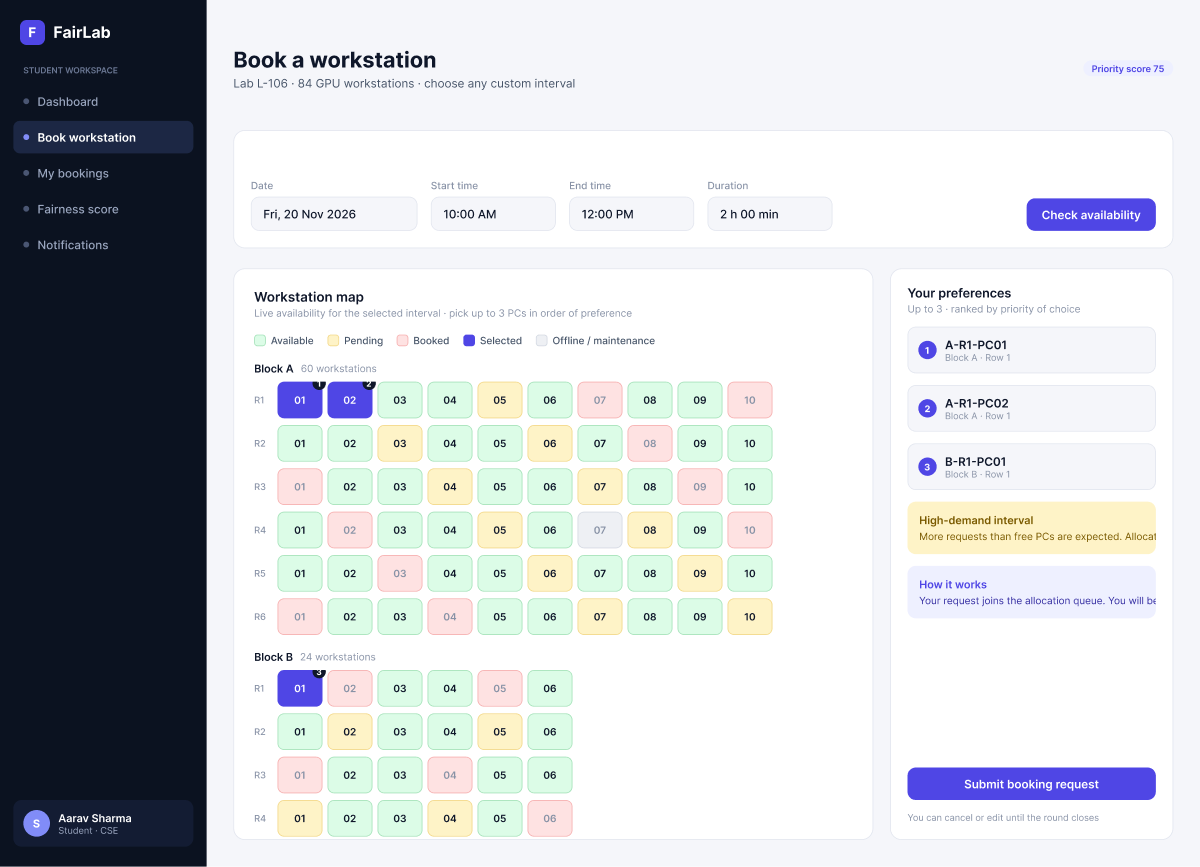
\includegraphics[width=0.92\linewidth]{ui_seatmap.png}
  \caption{FairLab student booking workspace showing the 84-workstation Lab L-106 map (Block~A $6\times 10$ + Block~B $4\times 6$), custom interval selector, and ranked preferences.}
  \label{fig:ui}
  \Description{Screenshot of the FairLab student Book Workstation interface showing the left navigation sidebar, date and time interval controls, color-coded 84-seat map separated into Block A and Block B, and the reservation summary panel.}
\end{figure}

\subsection{Database and Storage}
The normalized schema spans 18+ tables: \texttt{users} (including JSON \texttt{permissions}), \texttt{semesters}, \texttt{workstations}, \texttt{lab\_slots}, \texttt{booking\_requests}, \texttt{booking\_preferences}, \texttt{bookings}, \texttt{waitlist\_entries}, \texttt{student\_fairness}, \texttt{allocation\_rounds}, \texttt{allocation\_history}, \texttt{access\_passes}, \texttt{entry\_logs}, \texttt{notifications}, \texttt{outbox\_events}, \texttt{policy\_config}, \texttt{lab\_timetable}, \texttt{lab\_date\_overrides}, \texttt{ticket\_releases}, and \texttt{audit\_logs}. On the deployed campus VM, both Node.js replicas share \textbf{SQLite WAL} (\texttt{busy\_timeout=5000\,ms}, \texttt{foreign\_keys=ON}) with \texttt{BEFORE INSERT/UPDATE} overlap triggers and atomic outbox claiming (\texttt{UPDATE ... WHERE status='PENDING'}). A live \textbf{PostgreSQL 16.15} instance (\texttt{backend/db/postgres-schema.sql}) also runs on the VM with identical tables plus \texttt{btree\_gist} \texttt{EXCLUDE USING gist} overlap protection, validated by live PostgreSQL tests and ready for full async runtime cutover.

%% =====================================================================
\section{CSD Themes and Topics Applied in the Project}
\label{sec:csd-themes}
Table~\ref{tab:csd-themes} maps the Computer Systems Design concepts implemented in FairLab to their exact modules and engineering rationale.

\begin{table*}[t]
  \caption{Mapping of CSD themes and topics to their concrete implementation in FairLab}
  \label{tab:csd-themes}
  \footnotesize
  \setlength{\tabcolsep}{4.5pt}
  \renewcommand{\arraystretch}{1.18}
  \begin{tabularx}{\textwidth}{@{}p{0.17\textwidth}p{0.26\textwidth}X@{}}
    \toprule
    \textbf{Theme / Topic} & \textbf{Where Used in FairLab} & \textbf{Justification / Design Rationale} \\
    \midrule
    API Design & Versioned \texttt{/api/v1} REST + Zod~v4 + \texttt{Idempotency-Key} & Strict input schemas prevent malformed payloads; idempotency keys make client retries safe against duplicate bookings. \\
    Load Balancing & Nginx \texttt{least\_conn} across PM2 replicas (\texttt{:5000}, \texttt{:6000}) & Eliminates single-process bottleneck, provides automatic failover (\texttt{max\_fails=3}), and verifies cross-replica stateless JWT auth. \\
    Caching & 5\,s TTL \texttt{availabilityCache} + version counter & Avoids recomputing 84-seat occupancy on rapid map polls; invalidated on writes and cross-replica outbox tail events. \\
    Database Indexing \& Constraints & Composite indexes, SQLite triggers, PG16 \texttt{btree\_gist} & Enforces half-open $[start, end)$ non-overlap invariants atomically inside storage rather than trusting race-prone app checks. \\
    Concurrency \& Async Processing & Atomic \texttt{immediateTx}, WAL \texttt{busy\_timeout}, Transactional Outbox & Serializes competing requests inside ACID transactions and decouples crash-safe WebSocket delivery from booking commits. \\
    Monolith vs.\ Microservices & Layered Modular Monolith (2 replicas) & Appropriate for 84-seat campus scale; preserves single-DB ACID transactions without distributed-saga overhead. \\
    Design Patterns & Transactional Outbox, Strategy (3 fairness policies), Middleware Chain & Outbox guarantees at-least-once event propagation across crashes and replicas; middleware cleanly isolates auth, RBAC, and validation. \\
    Auth \& Authorization & HS256 JWT + \texttt{HttpOnly}/\texttt{Secure} cookie + 2-role/\texttt{ACCESS\_OPERATOR} & Zero client-trusted headers in production; least-privilege permission separates ordinary admins from physical gate operations. \\
    Deployment \& Ops & Campus VM (Nginx + PM2 daemon + PG16 + Ops Monitor) + Docker & Detached daemons survive SSH exit, auto-restart on \texttt{kill -9}, and provide live observability (\texttt{:7500}) and hot backups. \\
    Resilience \& Failure Handling & \texttt{SIGKILL} outbox recovery, maintenance reallocation, graceful shutdown & Pending outbox events recover on startup; taking a booked seat offline automatically moves active users to healthy seats. \\
    Algorithms \& Complexity & 4-tier fairness ranking ($O(R\log R)$) + preference matching ($O(R\cdot k)$) & Deterministic, fast ($<5\text{ ms}$ for 100 requests), mitigates starvation via waiting-time tie-breaking, and resists bot skew. \\
    Testing Strategy & 14 automated suites (concurrency, red-team, PG16, 50-seed, Phase~10) & Continuously verifies functional journeys, security boundaries, crash recovery, and statistical fairness metrics. \\
    \bottomrule
  \end{tabularx}
\end{table*}

\textbf{Deep Dive on Key Architectural Decisions:}
(1)~\textit{Transactional Outbox \& Cross-Replica WebSocket Scaling:} Because a shared database alone does not fan out in-memory WebSocket events between replicas, every replica runs a 1-second outbox tailer (\texttt{tailOutboxEventsSince}) that reads newly committed \texttt{outbox\_events} rows, invalidates its local availability cache, and broadcasts the deterministic \texttt{eventId} to its connected clients (measured $431\text{ ms}$ propagation from Replica~1 to Replica~2). Client-side deduplication prevents duplicate UI notifications, while backend mutations remain idempotent via \texttt{Idempotency-Key} and DB constraints.
(2)~\textit{Zero-Trust Identity \& Scoped Permissions:} Early design iterations used a client-provided \texttt{x-user-id} header and a third \texttt{watchman} role. Auditing exposed spoofing and role-model inconsistency risks; migrating every route to verified HS256 JWTs/cookies and replacing the third role with an \texttt{ACCESS\_OPERATOR} permission on designated admin accounts eliminated both weaknesses while keeping authorization simple.

%% =====================================================================
\section{Results and Evaluation}
\label{sec:results}
We evaluate FairLab across two dimensions: (a)~statistical fairness against a FIFO baseline across 50 deterministic Mulberry32 seeds (60 students, 10 slots/cycle, 4 workloads), and (b)~functional, security, concurrency, and crash-recovery verification across 14 automated test suites. Figure~\ref{fig:results} plots the measured 50-seed fairness results ($\mu \pm \sigma$). Under \textbf{Bot Latency Skew} (15\% automated scripts at 5--15\,ms vs.\ 85\% human users at 50--300\,ms), FIFO produces severe inequality (Gini $=0.657 \pm 0.009$, Jain's Index $=0.252 \pm 0.006$, max wait $=98.2$ cycles, $25.2\%$ relative under-allocation). FairLab lowers Gini by \textbf{96.7\%} to $0.022 \pm 0.002$, elevates Jain's Index to $0.998 \pm 0.0003$, cuts worst-case wait by \textbf{14.6$\times$} to $6.7$ cycles, and achieves $0\%$ starvation across all 50 seeds. Under 100\% \textbf{High Contention}, FairLab attains exact equality (Gini $=0.000$, Jain $=1.000$) when total slots divide evenly and Gini $=0.0098$ (Jain $=0.9996$) on non-divisible counts.

\begin{figure}[H]
  \centering
  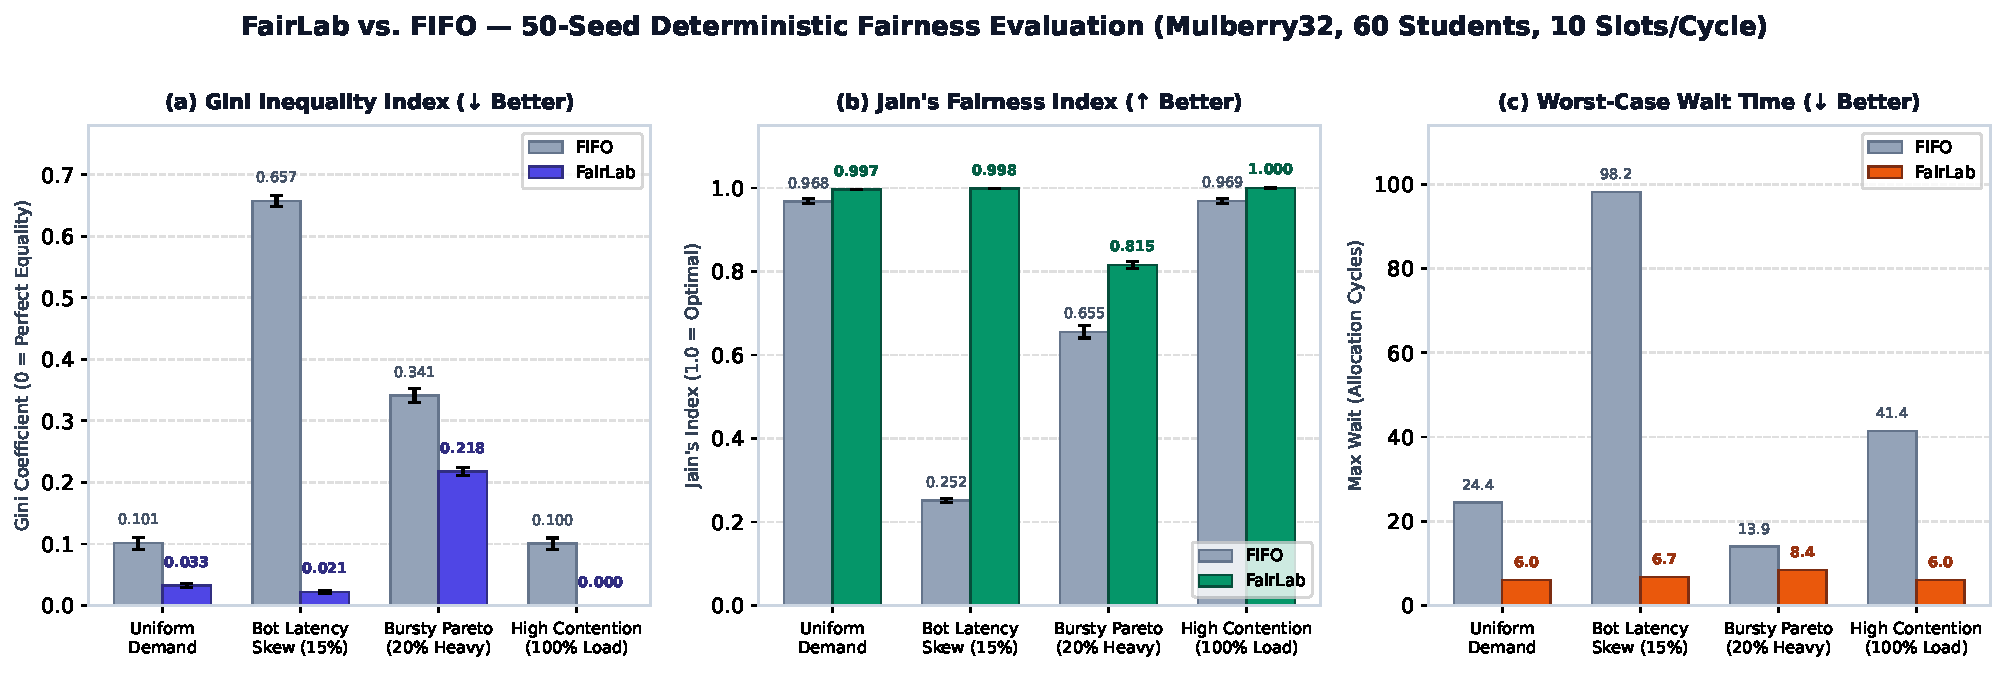
\includegraphics[width=0.98\linewidth]{fairlab_fairness_benchmark.pdf}
  \caption{50-seed deterministic fairness benchmark comparing FIFO vs.\ FairLab across four demand workloads: (a)~Gini inequality ($\downarrow$ better), (b)~Jain's Fairness Index ($\uparrow$ better), and (c)~worst-case wait cycles ($\downarrow$ better).}
  \label{fig:results}
  \Description{Three-panel grouped bar chart showing FairLab dramatically outperforming FIFO across Uniform, Bot Latency Skew, Bursty Pareto, and High Contention workloads, reducing Bot-Skew Gini from 0.657 to 0.021, raising Jain's index from 0.252 to 0.998, and cutting worst-case wait from 98.2 to 6.7 cycles.}
\end{figure}

\subsection{Performance}
Table~\ref{tab:performance} separates \textbf{measured test/deployment observations} from \textbf{projected capacity estimates}.

\begin{table}[htbp]
  \caption{Measured verification \& runtime performance vs.\ projected campus VM capacity}
  \label{tab:performance}
  \small
  \begin{tabularx}{\columnwidth}{@{}p{0.34\columnwidth}p{0.20\columnwidth}L@{}}
    \toprule
    \textbf{Metric / Scenario} & \textbf{Classification} & \textbf{Measured Result / Evidence} \\
    \midrule
    Master Automated Test Suite & Measured & \textbf{14/14 suites passing} (\texttt{tests/run-all-tests.js}); includes \textbf{76/76} Phase~10 acceptance assertions ($2.3\text{ s}$). \\
    100 Concurrent Requests vs.\ 5 Seats & Tested scenario & Completed in \textbf{172\,ms}; 5 top-score winners, 95 cleanly waitlisted, \textbf{0} duplicate seat assignments. \\
    6-Student Simultaneous \texttt{AUTO} Race & Tested scenario & \texttt{Promise.all} targeting \texttt{L106-PC-07}; \textbf{0} HTTP 500s, \textbf{0} double-bookings, 1-to-1 distinct assignments. \\
    Cross-Replica WS Propagation (VM) & Measured (live VM) & Booking on Replica~1 (\texttt{:5500}) received by Replica~2 WS client (\texttt{:6500}) in \textbf{431\,ms}. \\
    Hard \texttt{SIGKILL} Outbox \& PM2 Recovery & Measured (live VM) & SQLite WAL + startup outbox sweep recovered \texttt{PENDING} $\rightarrow$ \texttt{PUBLISHED}; PM2 restarted killed Replica~2 in \textbf{2\,s}. \\
    PostgreSQL~16 Live Operations & Measured (live VM) & \textbf{8/8} tests passing on PG~16.15 (\texttt{btree\_gist} \texttt{23P01} verified; \texttt{pg\_dump} 1,196 lines). \\
    VM Memory Footprint & Measured (live VM) & $\sim$78\,MB RSS per Node replica, 64\,MB ops monitor, 308\,KB JS bundle (80\,KB gzip). \\
    Campus Peak Capacity (500--2,000 users) & Capacity estimate & Projected $\sim$3.5\,GB peak RAM on 10\,vCPU / 10\,GB VM; requires formal k6 load test for SLA certification. \\
    \bottomrule
  \end{tabularx}
\end{table}

%% =====================================================================
\section{Discussion and Limitations}
\label{sec:discussion}
FairLab demonstrates that combining database-enforced half-open interval invariants, atomic contention detection, and history-aware fairness scoring eliminates FIFO bot dominance without sacrificing instant booking UX during off-peak periods. Several practical limitations remain and define our roadmap:
\begin{enumerate}
  \item \textbf{Active Runtime Database Split:} While PostgreSQL~16.15 runs live on the campus VM and passes all PostgreSQL verification suites, the live two-replica Express API currently shares SQLite WAL (\texttt{better-sqlite3}) because existing service modules use synchronous transaction calls. Migrating those calls to an async \texttt{pg} connection pool is straightforward future work for multi-host horizontal scaling.
  \item \textbf{Email Ownership \& Transport Security:} Checking the \texttt{@iitbhilai.ac.in} suffix filters domains, and demo accounts accept any non-empty password for academic demonstration; institutional production requires IIT Bhilai Google Workspace OAuth (\texttt{hd=iitbhilai.ac.in}) or LDAP/SSO plus HTTPS TLS termination at Nginx.
  \item \textbf{Hardware Integrations \& Load Certification:} Physical L-106 turnstile relays and NVIDIA-SMI workstation telemetry agents are intentionally decoupled (UI displays ``---'' honestly). Likewise, peak campus concurrency estimates should be validated with formal k6 load tests prior to institute-wide rollout.
\end{enumerate}

%% =====================================================================
\section{AI Tool Usage Declaration}
\label{sec:ai-usage}
During development, we used AI coding and design assistants (Antigravity / Gemini and Claude) for approximately 35--40\% of supporting effort, specifically for boilerplate UI/API scaffolding, iterative red-team security review, test-suite generation, diagram scripting, and LaTeX report editing. All system architecture decisions, fairness policy design, database schema invariants, security fixes, live campus VM deployment (Nginx load balancer, PM2 replicas, PostgreSQL~16), and final verification (14/14 automated test suites, 76/76 acceptance assertions, and live cross-replica tests) were independently reviewed, executed, debugged, and validated by the authors (Ganesh, V Karthik, and Charith Reddy).

%% =====================================================================
\appendix

\section{Source Code, Live Deployment, and Reproducibility}
\label{app:repo}
\begin{itemize}
  \item \textbf{GitHub Repository (Tag \texttt{v1.0.0}):} \url{https://github.com/gnshx/FAIR-LAB}
  \item \textbf{Live Campus VM Entry Point (Nginx Load Balancer + Frontend):} \url{http://10.1.75.40:3500}
  \item \textbf{Nginx Load Balancer Metrics:} \url{http://10.1.75.40:4500/lb-status}
  \item \textbf{Backend Replicas (Direct Health):} \url{http://10.1.75.40:5500/health} and \url{http://10.1.75.40:6500/health}
  \item \textbf{Live Operations \& Database Monitor:} \url{http://10.1.75.40:7500}
\end{itemize}

\textbf{Repository Layout:} \texttt{backend/} (Express server, middleware, 8 domain services, 6 route modules, SQLite WAL + PostgreSQL~16 schema/seed), \texttt{frontend/} (React~18 + Vite~6 + Tailwind 15-screen SPA), \texttt{tests/} (14 verification \& benchmark suites), and \texttt{docs/} (HLD/LLD, demo walkthrough, diagrams, release checklist).

\textbf{Reproducible Local Setup \& Full Test Execution:}
\begin{verbatim}
git clone https://github.com/gnshx/FAIR-LAB.git && cd FAIR-LAB
cd backend && npm install && cd ../frontend && npm install && npm run build
cd ../backend && node server.js     # Clean auto-seed (84 workstations) on :5000
node tests/run-all-tests.js         # Runs all 14 automated suites (100% pass)
node tests/test-phase10-validation.js # Standalone 76-assertion acceptance check
\end{verbatim}

\end{document}
\endinput
